\documentclass[12pt,a4paper,final]{article}
\usepackage[utf8]{inputenc}
\usepackage[russian]{babel}
\usepackage[OT1]{fontenc}
\usepackage{amsmath}
\usepackage{amsfonts}
\usepackage{amssymb}
\usepackage{hyperref}
\usepackage{graphicx}
\usepackage{xcolor}
\usepackage{tikz}
\usepackage{todonotes}

\usetikzlibrary{arrows,matrix,positioning}
\DeclareMathOperator{\rank}{rank}
\DeclareMathOperator{\diam}{diam}
\DeclareMathOperator{\ob}{Ob}
\DeclareMathOperator{\Hom}{Hom}
\DeclareMathOperator{\sign}{sign}
\DeclareMathOperator{\var}{Var}
\DeclareMathOperator{\bias}{Bias}
\newcommand{\sgn}{\text{sgn}}
\newcommand{\betah}{\hat{\bm \beta}}
\newcommand{\betaa}{\bm{\beta}}
\newcommand{\epss}{\bm{\varepsilon}}
\newcommand{\E}{\mathrm{E}}
\newcommand{\D}{\mathrm{D}}
\newcommand{\XT}{{\bm{X}}^{\mathrm{T}}}
\newcommand{\X}{\bm{X}}
\newcommand{\y}{\bm{y}}
\newcommand{\1}{\mathds{1}}
\newcommand{\prob}{\mathrm{P}}
\DeclareMathOperator*{\argmax}{arg\,max}
\DeclareMathOperator*{\argmin}{arg\,min}
\newtheorem{definition}{Определение}
\newtheorem{theorem}{Теорема}
\usepackage{bm}
\usepackage[left=2cm,right=2cm,top=2cm,bottom=2cm]{geometry}


\newtheorem{proposition}{Предложение}


\author{Дейвид Капаца, Анастасия Мандрикова, Елена Гоголева}
\title{Регрессия, регуляризация, отбор признаков}
\begin{document}
\maketitle
\tableofcontents

\newpage
%
%\subsection{Требования к докладам}
%
%\begin{enumerate}
%\item Какая практическая задача решается. Пример данных, на основе которых предполагается ее решать.
%\item Если обучение без учителя, то используется базовая модель данных. В этом случае, скорее всего, будет максимизироваться функция правдоподобия. Если с учителем, то используется модель (алгоритм) предсказания и мера для ошибки предсказания, которая будет минимизироваться.
%\item Дальше, теоретически, просто оптимизационная задача и обсуждение метода ее решения. Например, в случае без учителя это м.б. EM-алгоритм. В случае с учителем – метод стохастического градиента. При этом, если исходно в задаче были условия, при сведении задачи к безусловной оптимизации используются теорема Лагранжа или теорема Куна-Такера.
%\item Обсуждение свойств метода оптимизации. Улучшение алгоритма за счет специфики задачи, эвристических приемов.
%\item Возможная регуляризация, которую можно рассматривать как просто изменение оптимизационной задачи в той же модели с целью получать оценки параметров с лучшими свойствами; в частности, для получения нулевых оценок в случае добавления модуля параметра.
%\item Изменение (усложнение или упрощение) рассматриваемой модели данных или предсказывающего алгоритма и переход к пункту 3.
%\item Примеры (могут перемежаться с теорией).
%\end{enumerate}
%
%\subsection{Требования: теория}
%
%\begin{enumerate}
%\item Внятно рассказана математическая постановка задачи.
%\item Описан бэкграунд задачи (частным случаем чего является, в чем особенность и пр.)
%\item Приведены и формализованы примеры, соответствующие этой постановке задачи.
%Описан и объяснен метод решения задачи.
%\item Приведено математическое обоснование метода (привести теор.результат и объяснить).
%\item Приведен (с объяснением) алгоритм решения задачи.
%\item Объяснены особенности реализации алгоритма.
%\item При рассказе понятно, что в данный момент обсуждается, постановка задачи, алгоритм решения, проблемы реализации алгоритма, \dots
%\item Рассказано, какие проблемы существуют в данном методе/алгоритме и какие есть пути их разрешения.
%\end{enumerate}
%
%\subsection{Требования: практика}
%
%\begin{enumerate}
%\item Проведено сравнение методов/моделей.
%\item Понятно, почему выбраны такие метод/параметры.
%\item Понятно, как идет контроль за отсутствием переподгонки и как оценивается точность.
%\item Понятно, как интерпретируются результаты.
%\item Объяснен код/функции, которые используются в примере.
%\end{enumerate}

\section{Регрессия в ML и вероятностная модель}

Сначала о том, какую задачу мы хотим решить и какие минимальные условия следует наложить на данные для того, чтобы она была решаемой.

Пусть имеется некоторый набор данных (обучающая выборка):
\begin{enumerate}
  \item $\X \in \mathbb R^{n \times p}$ --- матрица данных, матрица плана (data matrix, design matrix), состоит из столбцов $X_i$ (признаки) и строк $\mathbf x_i$ (индивиды, объекты); 
  \item $\y \in \mathbb R^n$ --- ответ, вектор наблюдений (response vector). 
\end{enumerate}
\textbf{\color{blue}{Задача регрессии:}}

\colorbox{yellow}{\parbox{\textwidth}{ Уметь предсказывать $y_i$ (ответы) по \textit{новым} $\mathbf x_i$ (объектам, индивидам), установив некоторую зависимость на обучающей выборке. }}
\vskip 0.2 in 
\subsection{ML подход: гипотеза непрерывности}
\noindent Какими должны быть данные для того, чтобы данная задача была корректной? Нужно, чтобы все рассматриваемые объекты были в некотором смысле однородны и происходили из некоторой генеральной совокупности (если иначе, то как предсказать ответ, когда новый объект $\mathbf x_i$ совершенно не похож на объекты обучающей выборки).

В машинном обучении для обоснования использования методов регрессии используется так называемая \textbf{гипотеза непрерывности}:

\colorbox{yellow}{\parbox{\textwidth}{ <<близким>> объектам $\mathbf x_i$ соответствуют <<близкие>> ответы $y_i$}}
\vskip 0.2 in 

\noindent Такая гипотеза, несмотря на свою простоту и наглядность, допускает множество интерпретаций и имеет свои недостатки.
Пожалуй, главная проблема заключается в полном отсутствии случайности.\footnote{Если объект и ответ регистрируются со случайной ошибкой, то мы уже не можем сказать, что одинаковые объекты приводят к одинаковым ответам. Но тогда получаем противоречие с гипотезой непрерывности.} 
Можно формализовать задачу регрессии на вероятностном языке. Приведём один из вариантов.

\subsection{Вероятностная постановка задачи регрессии}
Пусть $\bm \xi \in \mathbb R^p$ --- случайный вектор, $\eta, \varepsilon \in \mathbb R$ --- случайные величины.

Предполагаем, что $\eta$ и $\bm \xi$ функционально зависимы: 
\begin{equation}
  \eta = \varphi(\bm \xi) + \varepsilon.
\end{equation}
Обычно $\E \varepsilon = 0, \, \D \varepsilon = \sigma^2,\, \bm\xi \perp \varepsilon$; часто имеют место предположения о распределении $\varepsilon$. 

Задачей в данном случае является нахождение функции $\bm \varphi$.
Переходя к выборке, наблюдаем $\mathbf x_1, \ldots, \mathbf x_n \sim \mathcal L(\bm \xi)$ и $y_1, \ldots, y_n \sim \mathcal L(\eta)$. На основании этой выборки делаем предположение о $\bm \varphi$, получаем её приближение $\hat{\bm{\varphi}}$. Предсказанием ответа $\tilde y$ для нового объекта $\tilde{\mathbf{x}}$ на построенной модели будет $\hat{\bm{\varphi}}(\tilde{\mathbf{x}}).$  

Таким образом, с помощью вероятностного подхода удаётся формализовать задачу и получить удобную для построения и анализа модели вероятностную интерпретацию. Далее мы рассмотрим стандартные этапы обучения модели с учителем, которые применяются и в регрессионной постановке.

\subsection{Этапы обучения модели}

Так как тема регрессии в целом предполагается неплохо знакомой, а доклад является вводным в тематику обучения с учителем, напомним классическую схему обучения модели. Каждый из этапов приведён с соответствующим примером (случай классической линейной регрессии).

\begin{enumerate}
	\item \textbf{Выбор модели регрессии} (класс рассматриваемых $\varphi(\cdot)$)
	
	{\color{gray} Линейная модель: $\varphi(\mathbf x_i, \betaa) = \sum_{j = 1}^p \beta_i \mathbf x_i[j],\quad i \in 1:n $}
	
	Чаще всего на практике в качестве кандидатов на $\bm \varphi$ рассматривается именно класс линейных функций. Такой выбор обусловлен явным видом решения во многих случаях, его простотой и повышенной интерпретируемостью.
	
	\item \textbf{Выбор функции потерь} (loss function)
	
	{\color{gray} Квадратичная функция потерь: $\sum_{i = 1}^n(y_i - \varphi(\mathbf x_i, \betaa))^2$}
		
		Значение функции потерь отражает качество рассматриваемой модели на тренировочной выборке, измеряя отличие между предсказаниями $\tilde y_i$ и наблюдениями $y_i$. Вариант по умолчанию ---  сумма квадратов остатков --- обусловлен своей простотой и дифференцируемостью, а также тем, что он естественно возникает при предположении о нормальном распределении остатков $\bm \varepsilon$. 
	
	\item \textbf{Выбор метода обучения} (training)

{\color{gray} МНК: $\betah = \argmin_{\betaa}{\sum_{i = 1}^n(y_i - \varphi(\mathbf x_i, \betaa))^2}$}

		Обучение модели представляет из себя задачу нахождения наилучшей модели среди рассматриваемых (например, заданных семейством параметров $\betaa$). Обычно такой выбор происходит за счёт минимизации функции потерь. В указанном случае линейной регрессии решение находится явно, однако так получается не всегда. В зависимости от вида функции потерь приходится использовать различные методы оптимизации (градиентные, если есть производная; стохастические, если функция сложная; условные, если на параметры накладываются некоторые ограничения, и т.д.). Также обращают внимание на свойства полученной оценки: в указанном примере получаем наилучшую несмещённую оценку вектора коэффициентов (BLUE). 
		
	\item \textbf{Выбор метода проверки} (test)

{\color{gray} MSE: $\tfrac{1}{n_{\text{test}}}\sum_{i = 1}^{n_{\text{test}}}(y^{\text{test}}_i - \varphi(\mathbf x_i^{\text{test}}, \betah))^2$}

Для оценки качества построенной модели и сравнения модели с другими построенными используется тестовая выборка, в нашем случае это mean-squared error. Сравнение величин ошибок на тестовой и на тренировочной выборке может оказаться полезным для выявления проблемы переобучения: низкая ошибка при тренировке и высокая при тестировании могут свидетельствовать о наличии этой проблемы.

\end{enumerate}            

Далее мы подробнее остановимся на некоторых этапах.

\section{Задача регрессии как задача оптимизации}

Задача параметрической\footnote{непараметрическую мы не рассматриваем ввиду того, что с ней сложнее предсказывать} регрессии может быть сформулирована как задача минимизации некоторого функционала от выборки.
Рассмотрим такую формулировку.

 Пусть заданы:
\begin{itemize}
	\item $\X \in \mathbb R^{n \times p}$ --- матрица данных (design matrix);
	\item $\bm y \in \mathbb R^n$ --- вектор ответов;
	\item $\betaa \in \mathbb R^d$ --- вектор параметров;
	\item $\bm \varphi(\X, \betaa) := (\varphi(\mathbf x_1, \betaa),\ldots, \varphi(\mathbf x_n, \betaa) )^\mathrm T$ --- функция от выборки и параметров;	\item $\mathcal L(\bm \varphi(\X, \betaa), \bm y)$ --- \textit{некоторая} функция потерь.\footnote{здесь
	$\mathcal L: \mathbb R^{n} \times \mathbb R^n \rightarrow \mathbb R$
	}
\end{itemize}

Тогда решением задачи регрессии будет вектор $\betah$:

$$\betah = \argmin_{\betaa}{\mathcal L(\bm \varphi(\X, \betaa), \bm y)}.$$

Такая запись сразу позволяет увидеть, что мы имеем дело с некоторой оптимизационной задачей. Минимизация функции $\mathcal L(\bm \varphi(\X, \betaa), \bm y)$ на некотором пространстве параметров приводит к оптимальному решению.\footnote{конечно, можно вводить ограничения на пространство (например, исходя из смысла задачи, можно рассматривать только положительные $\betah$), но в данном случае для простоты рассматриваем безусловную оптимизацию} 

В редких случаях удаётся найти явное решение,\footnote{например, в случае линейной регрессии при выборе суммы квадратов остатков в качестве функции потерь} однако в общем случае решение находится приближённо с использованием методов приближённых вычислений, поэтому помимо статистической ошибки полученного результата следует учитывать и вычислительную погрешность, которая зависит от выбранного метода оптимизации, точности входных данных, а также момента остановки алгоритма.

Также нельзя забывать и про то, что при использовании некоторых методов численной оптимизации есть шанс попасть не в глобальный, а в локальный минимум или седловую точку, что приведёт к неудовлетворительной оценке $\betah.$ Применяя ту и иную функцию оптимизации, следует проверить наличие ограничений или условий для сходимости алгоритма.

\section{Выбор функции потерь}

Выбор функции потерь $\mathcal L$ несёт критическую роль в решении задачи регрессии, поэтому он должен быть обоснован каждый раз, когда решается та или иная задача.
Есть множество вариантов функций потерь для разных задач, в качестве примеров перечислим три из них, которые хорошо изучены и имеют свои применения в разных условиях:
\begin{itemize}
	\item $\|\bm \varphi(\bm X, \betaa) - \bm y\|^2_2$ --- квадратичная ошибка ($l_2$-норма);
	\item $\|\bm \varphi(\bm X, \betaa) - \bm y\|_1$ --- модуль ошибки ($l_1$-норма);
	\item $\sum_{i \in 1:n} H_\delta(\varphi(\mathbf x_i, \betaa), y_i)$ --- функция потерь Хубера, 
	
	где $H_\delta$ --- функция Хубера, квадратичная на $[-\delta, \delta]$ и линейная на $|x|>\delta$.
\end{itemize}


\paragraph{Как выбирать?}

Выбор должен быть основан на нескольких критериях, вот их приблизительная подборка (приоритет пунктов определяется в зависимости от конкретной задачи):

\begin{itemize}
	\item Явный вид решения;
	\item Простота функции $\mathcal L$ для оптимизации;
	\item Точность данных/наличие выбросов;
	\item Конкретные предположения о распределении остатков $\bm \varepsilon$;
	\item Инвариантность решения относительно масштаба/сдвига для признаков.
\end{itemize}
В дальнейшем осветим эти пункты подробнее на примере линейной регрессии.

\section{Линейная регрессия}

Частным случаем задачи регрессии является линейная регрессия. Мы делаем предположение о том, что модель данных имеет следующий вид:
\begin{equation}
	\bm y = \X \betaa + \epss,
\end{equation}
где 
\begin{itemize}
	\item $\bm y \in \mathbb R^n$ --- вектор ответов,  $\epss \in \mathbb R^n$ --- вектор ошибок, $\mathrm E\epss = \bm 0$;
	\item $\X \in \mathbb R^{n \times p}$ --- матрица данных (design matrix):
	\begin{itemize}
	\item детерминированная (для простоты рассматриваем этот случай, то есть предполагаем, что случайность в модели происходит только от вектора шума);
	\item случайная (результаты похожи, но уже с условными математическими ожиданиями из-за случайности матрицы, здесь не будем рассматривать);
	\end{itemize}		
	\item $\betaa \in \mathbb R^p$ --- вектор параметров;
	\item $n\geqslant p.$
	\end{itemize}
	
Заметим, что такое предположение обосновано не только простотой результирующей модели. Если столбцы матрицы $\X$ (то есть признаки) и вектор $\y$ распределены нормально, то известно, что $\y$ является \textit{линейной} 	комбинацией столбцов матрицы $\X$.


На случайную ошибку обычно накладываются следующие требования:
\begin{equation}
  \E \varepsilon_i = 0,\, \E \varepsilon_i^2 = \sigma^2 < +\infty,\,  \E \varepsilon_i \varepsilon_j = 0.
\label{req:err}
\end{equation}
Решение задачи линейной регрессии --- вектор $\betah$. 

Если не оговорено иное, под задачей линейной регрессии подразумевается задача минимизации квадратичной функции потерь:

\textbf{Классическая задача}:

$$\betah = \argmin_{\betaa}{\|\bm y - \bm X \betaa\|^2_2}.$$

Полученную оценку $\betah_{\text{МНК}}$ называют оценкой по методу наименьших квадратов (МНК-оценкой). Она имеет явный вид (если матрица $\XT \X$ невырожденная):\footnote{берутся частные производные по компонентам вектора $\betaa$ функции потерь и приравниваются к нулю. В результате получаем уравнение, которое и даёт указанную оценку.}
\begin{equation}
  \betah_{\text{МНК}} = (\XT \X)^{-1}\XT \y.
  \label{eq:lse}
\end{equation}

Сразу отметим, что наличие явного вида решения крайне удобно в вычислительном плане. 
Оценка вычисляется достаточно быстро посредством применения сингулярного разложения матрицы данных $\X$, в чём мы убедимся далее.

\subsection{Особенности МНК-оценки}

В данном разделе отметим основные особенности оценки (\ref{eq:lse}).

Начнём с математического ожидания и дисперсии оценки (напомним, что действуем в предположении, что матрица $\X$ --- детерминированная). Математическое ожидание вычислим прямо здесь:
\begin{multline}
	\E \betah_{\text{МНК}} = \E [(\XT \X)^{-1}\XT \y] = (\XT \X)^{-1}\XT \E \y = (\XT \X)^{-1}\XT \E (\X \betaa + \epss) = \\ = (\XT \X)^{-1}\XT \E (\X \betaa) + (\XT \X)^{-1}\XT \underbrace{\E \epss}_{= 0}) = (\XT \X)^{-1}\XT \E (\X \betaa) = \\ = \underbrace{(\XT \X)^{-1}(\XT\X)}_{= \mathbf I}\betaa = \betaa
\end{multline}
Таким образом, мы показали, что оценка $\betah_{\text{МНК}}$ является \textit{несмещённой}. 

С дисперсией (ковариационной матрицей, если точнее) чуть посложнее, поэтому просто выпишем результат (при условии выполнения требований (\ref{req:err})):
\begin{equation}
  \D {\betah_{\text{МНК}}} = \sigma^2 (\XT\X)^{-1}.
  \label{eq:var}
\end{equation}
\textit{Теорема Гаусса--Маркова} утверждает, что $\betah_{\text{МНК}}$ имеет наименьшую дисперсию среди всех несмещённых оценок (best linear unbiased estimate --- BLUE). Таким образом, у найденной оценки отсутствует смещение, и в то же время она имеет наименьшую дисперсию среди всех возможных оценок.


Хорошая оценка $\betah$ должна иметь низкую среднеквадратическую\footnote{это один из наболее распространённых критериев того, что выбранная оценка является наилучшей. К примеру, выборочное среднее является решением задачи минимизации среднеквадратической ошибки $\min_{a}\frac{1}{n}\sum_{i = 1}^n (x_i - a)^2$} ошибку $\E (\betaa - \betah)^2$, а она раскладывается в следующую сумму:
\begin{equation}
\label{eq:mse}
\E(\betaa - \betah)^2 = \underbrace{\mathrm D \betah}_{\text{дисперсия}} + \underbrace{(\mathrm E \betah - \betaa)^2}_{\text{смещение}}.
\end{equation}
Отсюда становится видно, что обе характеристики --- дисперсия и смещение --- одинаково важны для получения наилучшей оценки и что несмещённая оценка всё же может иметь больш\'{у}ю среднеквадратичную ошибку из-за достаточно большой дисперсии. О том, как можно уменьшить среднеквадратическую ошибку за счёт допущений на смещение оценки, мы поговорим в разделе \ref{sec:reg}.

Также добавим, что полученная оценка $\betah_{\text{МНК}}$ (при выполении условий (\ref{req:err}) и нормальности ошибок) является оценкой по методу максимума правдоподобия (ОМП), что позволяет говорить об асимптотической нормальности и асимптотической эффективности $\betah_{\text{МНК}}$.

\subsection{Распределение ошибки в модели}
Если ошибки удовлетворяют данным в (\ref{req:err}) условиям, а также распределены по нормальному закону, МНК-оценка является BLUE и ОМП. В таком случае использование  хорошо известных на практике критериев о значимости регрессии является корректным.

Однако, такие требования выполняются не всегда. Данные могут иметь выделяющиеся наблюдения (outliers), а ошибки могут быть распределены не нормально; также, при отклонении от линейной модели возможно возникновение проблемы гетероскедастичности. 

В таком случае становится необходимостью использование других функций потерь и других методов оптимизации. Говорить о явном решении уже не приходится, однако на практике применение таких подходов приводит к более устойчивым и лучшим в плане среднеквадратической ошибки оценкам.

\subsection{Вычисление МНК-оценки: сингулярное разложение}

В этом разделе покажем, как используется сингулярное разложение матрицы для упрощения задачи вычисления $\betah_{\text{МНК}}$, а затем обсудим вопросы вычислительной устойчивости полученной оценки.

Напомним некоторые необходимые факты про сингулярное разложение. \textit{Сингулярным разложением} матрицы $\X$ называется разложение $\X = \bm V \bm D \bm U^\mathrm T$, где
\begin{itemize}
\item $\bm V$ и $\bm U$ --- ортогональные,\footnote{основное свойство ортогональных матриц: $\bm V^\mathrm T =\bm V^{-1}$ (используется при выводе формулы для $\betah_{\text{МНК}}$)} $\bm D$ --- диагональная;
\item $\bm V = (V_1, V_2, \ldots, V_n) \in \mathbb R^{n\times n}$, $V_i$ --- собственные векторы $\X \XT$;
\item $\bm U = (U_1, U_2, \ldots, U_n) \in \mathbb R^{p\times n}$, $U_i$ --- собственные векторы $\XT \X$;
\item $\bm D = \mathrm{diag}(\sqrt{\lambda_1}, \ldots,\sqrt{\lambda_n})$, $\lambda_j \geqslant 0$ --- собственные значения $\XT \X$.
\end{itemize}
Для простоты предположим, что имеем дело с матрицей полного ранга, $p = n$ (результаты распространяются на случай $n>p$).

Подставим в формулу для $\betah_{\text{МНК}}$ вместо матрицы $\X$ её сингулярное разложение и получим
\begin{multline}
  \label{eq:sing}
  \betah_{\text{МНК}} =\\= (\XT \X)^{-1}\XT \y = (\bm U \bm D \bm V^\mathrm T \bm V \bm D \bm U^\mathrm T)^{-1} \bm U \bm D \bm V^\mathrm T \y = (\bm U \bm D \bm V^{-1} \bm V \bm D \bm U^\mathrm T)^{-1} \bm U \bm D \bm V^\mathrm T \y = \\
  = (\bm U \bm D^2 \bm U^\mathrm T)^{-1} \bm U \bm D \bm V^\mathrm T \y = \bm U \bm D^{-2} \bm U^\mathrm T \bm U \bm D \bm V^\mathrm T \y =\\= \bm U \bm D^{-1} \bm V^\mathrm T \y,
\end{multline}
где $\bm D^{-1} = \mathrm{diag} (1/\sqrt{\lambda_1}, \ldots, 1/\sqrt{\lambda_n})$.
Если предположить, что вычисление сингулярного разложения на компьютере происходит быстро и с малой погрешностью (в целом так и есть), то такой подход к вычислению $\betah_{\text{МНК}}$ оказывается наиболее предпочтительным.

\subsection{Мультиколлинеарность} 
Подход с сингулярным разложением также позволяет пролить свет на одну из главных проблем в задаче регрессии --- проблему коллинеарности признаков (столбцов матрицы $\X$).

Обратим внимание на разложение (\ref{eq:sing}). Формула для $\betah_{\text{МНК}}$ содержит матрицу $\bm D^{-1} = \mathrm{diag} (1/\sqrt{\lambda_1}, \ldots, 1/\sqrt{\lambda_n})$, состоящую из корней собственных чисел $\XT \X$. Ясно, что когда собственные числа оказываются приближённо равными нулю, возникает проблема вычислительной неустойчивости, когда погрешность вычислений может возрасти существенно. В таком случае говорят, что матрица $\XT \X$ близка к вырожденной или плохо обусловлена.

\paragraph{Когда собственные значения $\XT \X$ малы?}
~\\Ответ на этот вопрос можно получить из следующего факта:
\vskip 0.1 in 
\noindent
\colorbox{yellow}{\parbox{\textwidth}{ Если существует $\bm v \in \mathbb R^p$ такой, что $\X \bm v \approx \bm 0$, то некоторые $\lambda_i \approx 0$. }}
\vskip 0.1 in 
\noindent Таким образом, когда некоторые из признаков близки к коллинеарным, некоторые собственные числа становятся близкими к нулю. Следующее определение формализует данную проблему.
\begin{definition}
$\mu(\bm S) = \|\bm S\|\|\bm S^{-1}\| = {\lambda_{\text{max}}}/{\lambda_{\text{min}}}$ называется \textbf{числом обусловленности} матрицы $\bm S$
\end{definition}

Ещё один известный факт\footnote{любой учебник по вычислительным методам и теории приближённых вычислений в линейной алгебре} состоит в том, что при вычислении $\bm S^{-1}\bm v = \bm z$ (что, вообще говоря, и делается при подсчёте оценки $\betah_{\text{МНК}}$) происходит увеличение погрешности в $\mu(\bm S)$ раз:
$$
\frac{\|\delta \bm z\|}{\|\bm z\|} \leqslant \mu(\bm S) \frac{\|\delta \bm v\|}{\|\bm v\|}
$$

Помимо вычислительной, у проблемы мультиколлинеарности есть и статистическая сторона. Напомним, что дисперсия оценки $\betah_{\text{МНК}}$ вычисляется по формуле (\ref{eq:var}):
$$
  \D {\betah_{\text{МНК}}} = \sigma^2 (\XT\X)^{-1}.
$$
Норма полученной матрицы увеличивается с увеличением коллинеарности ($\|(\XT\X)^{-1}\|_2 = \lambda_{min}^{-1}$), что свидетельствует об увеличении дисперсии оценки $\betah_{\text{МНК}}$. Это, в свою очередь, автоматически приводит к увеличению MSE, что негативно сказывается на точности и предсказательной силе.

Таким образом, проблема мультиколлинеарности приводит как к проблеме вычислительной неустойчивости, так и к увеличению дисперсии у полученной оценки. Существует несколько методов борьбы с этой проблемой:
\begin{itemize}
	\item Уменьшение числа признаков (отбор признаков) (см. \ref{sec:sel});
	\item Регуляризация (см. \ref{sec:reg});
	\item Преобразование признаков (Анализ главных компонент и т.п., в данном докладе не рассматривается).
\end{itemize}
В следующих разделах мы подробнее рассмотрим другие модификации и методы регрессии, и увидим, что они в той или иной мере помогают решить эту и остальные приведённые выше проблемы МНК-оценок.

\section{Регуляризация в линейной регрессии}
\label{sec:reg}
Как уже говорилось ранее, одним из главных критериев качества оценки является MSE, разложение которого имеет вид (\ref{eq:mse})
$$
\E(\betaa - \betah)^2 = \underbrace{\mathrm D \betah}_{\text{дисперсия}} + \underbrace{(\mathrm E \betah - \betaa)^2}_{\text{смещение}}.
$$
И так как мы рассмотрели МНК-оценку, которая имеет наименьшее смещение, но \textit{не гарантирует} минимизацию всего MSE, можно попробовать допустить смещение и надеяться на то, что за счёт уменьшения дисперсии MSE удастся уменьшить. 

Модель остаётся той же, то есть остаёмся в контексте линейной регрессии и предполагаем выполнение условий \ref{req:err}:
$$
\bm y = \X \betaa + \epss
$$

\subsection{Гребневая регрессия}
	
Возьмём оценку по МНК и сделаем её смещённой, добавив к матрице $\XT \X$ слагаемое $\lambda \mathbf I$, где $\lambda > 0$ --- параметр, регулирующий смещение:
\begin{equation}
\label{eq:ridge}
  \betah_{\text{ridge}} = (\XT \X + \lambda \mathbf I)^{-1}\XT\bm y,\quad \lambda > 0.
\end{equation}
	Если расписать данную оценку с помощью SVD, получим
	$$\betah_{\text{ridge}} = \sum_{i = 1}^n \frac{\sqrt{\lambda_j}}{\lambda_j + \lambda} U_j(V_j^\mathrm T\bm y).$$
За счёт положительного параметра $\lambda >0$ получается отделить знаменатель от нуля. То есть устойчивость вычислений повышается. 

Что происходит с дисперсией оценки? Исходя из вида коэффициента
$$
\frac{\sqrt{\lambda_j}}{\lambda_j + \lambda},
$$
можно заметить, что параметром $\lambda > 0$ штрафуются все компоненты, но в особенности те, которые малы, что уменьшает дисперсию оценки.

На рис.\,\ref{fig:rid} хорошо видно, как с изменением $\lambda$ достигается компромисс между дисперсией и смещением. Однако такой график для реальных данных мы получить не можем, так как изначально неизвестно, чему равно смещение и дисперсия оценки.
Чаще всего \textbf{выбор параметра} $\lambda$ осуществляется на основании кросс-валидации, то есть минимизации ошибки на валидационной выборке (есть и теоретические оценки, но они зависят от многих параметров, поэтому обычно не используются). 

\begin{figure}[]
\centering
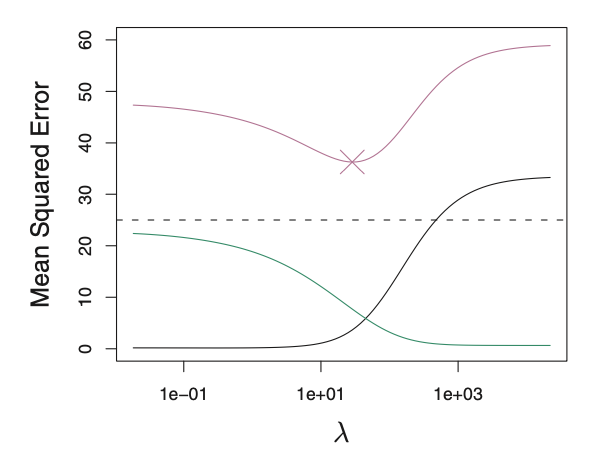
\includegraphics[width=0.5\textwidth]{ridge2.png}
\caption{Пример для сгенерированных данных. По оси $x$ отложены значения параметра регуляризация $\lambda$. Зелёная кривая --- дисперсия оценки, чёрная --- её смещение, среднеквадратическая ошибка с обозначенным минимумом --- красная.}
\label{fig:rid}
\end{figure}

Задача, явное решение которой записано в (\ref{eq:ridge}), называется задачей \textit{гребневой регрессии} (ridge regression). Она может быть сформулирована двумя эквивалентными способами
\begin{equation}
\label{eq:rid1}
 \betah_{\text{ridge}}(\mu) = \argmin_{\betaa}{\|\bm y - \X\betaa\|^2_2 +\mu \|\betaa\|^2_2}, \quad \mu >0,
\end{equation}
\begin{equation}
\label{eq:rid2}
\betah_{\text{ridge}}(\lambda) = \argmin_{\betaa}{\|\bm y - \X\betaa\|^2_2 \text{, т.ч. } \|\betaa\|^2_2 \leqslant \lambda}, \quad \lambda >0.
\end{equation}
Заметим, что $\lambda$ и $\mu$ при равенстве не дают одинаковых задач: $\mu = \infty$ и $\lambda = 0$ приводят к нулевой оценке $\betah_{\text{ridge}} = \bm 0$, а $\mu = 0$ и $\lambda = \infty$ приводят к классической оценке по МНК.

По ссылке \url{https://www.desmos.com/calculator/3fp4awzeyp}
можно посмотреть на геометрическое построение задачи (\ref{eq:rid2}) в случае, когда $n = p = 2$, то есть оси --- значения двумерного вектора $\betaa$. На рисунке \ref{fig:rid_des} --- пример такого построения.
\begin{figure}[]
\centering
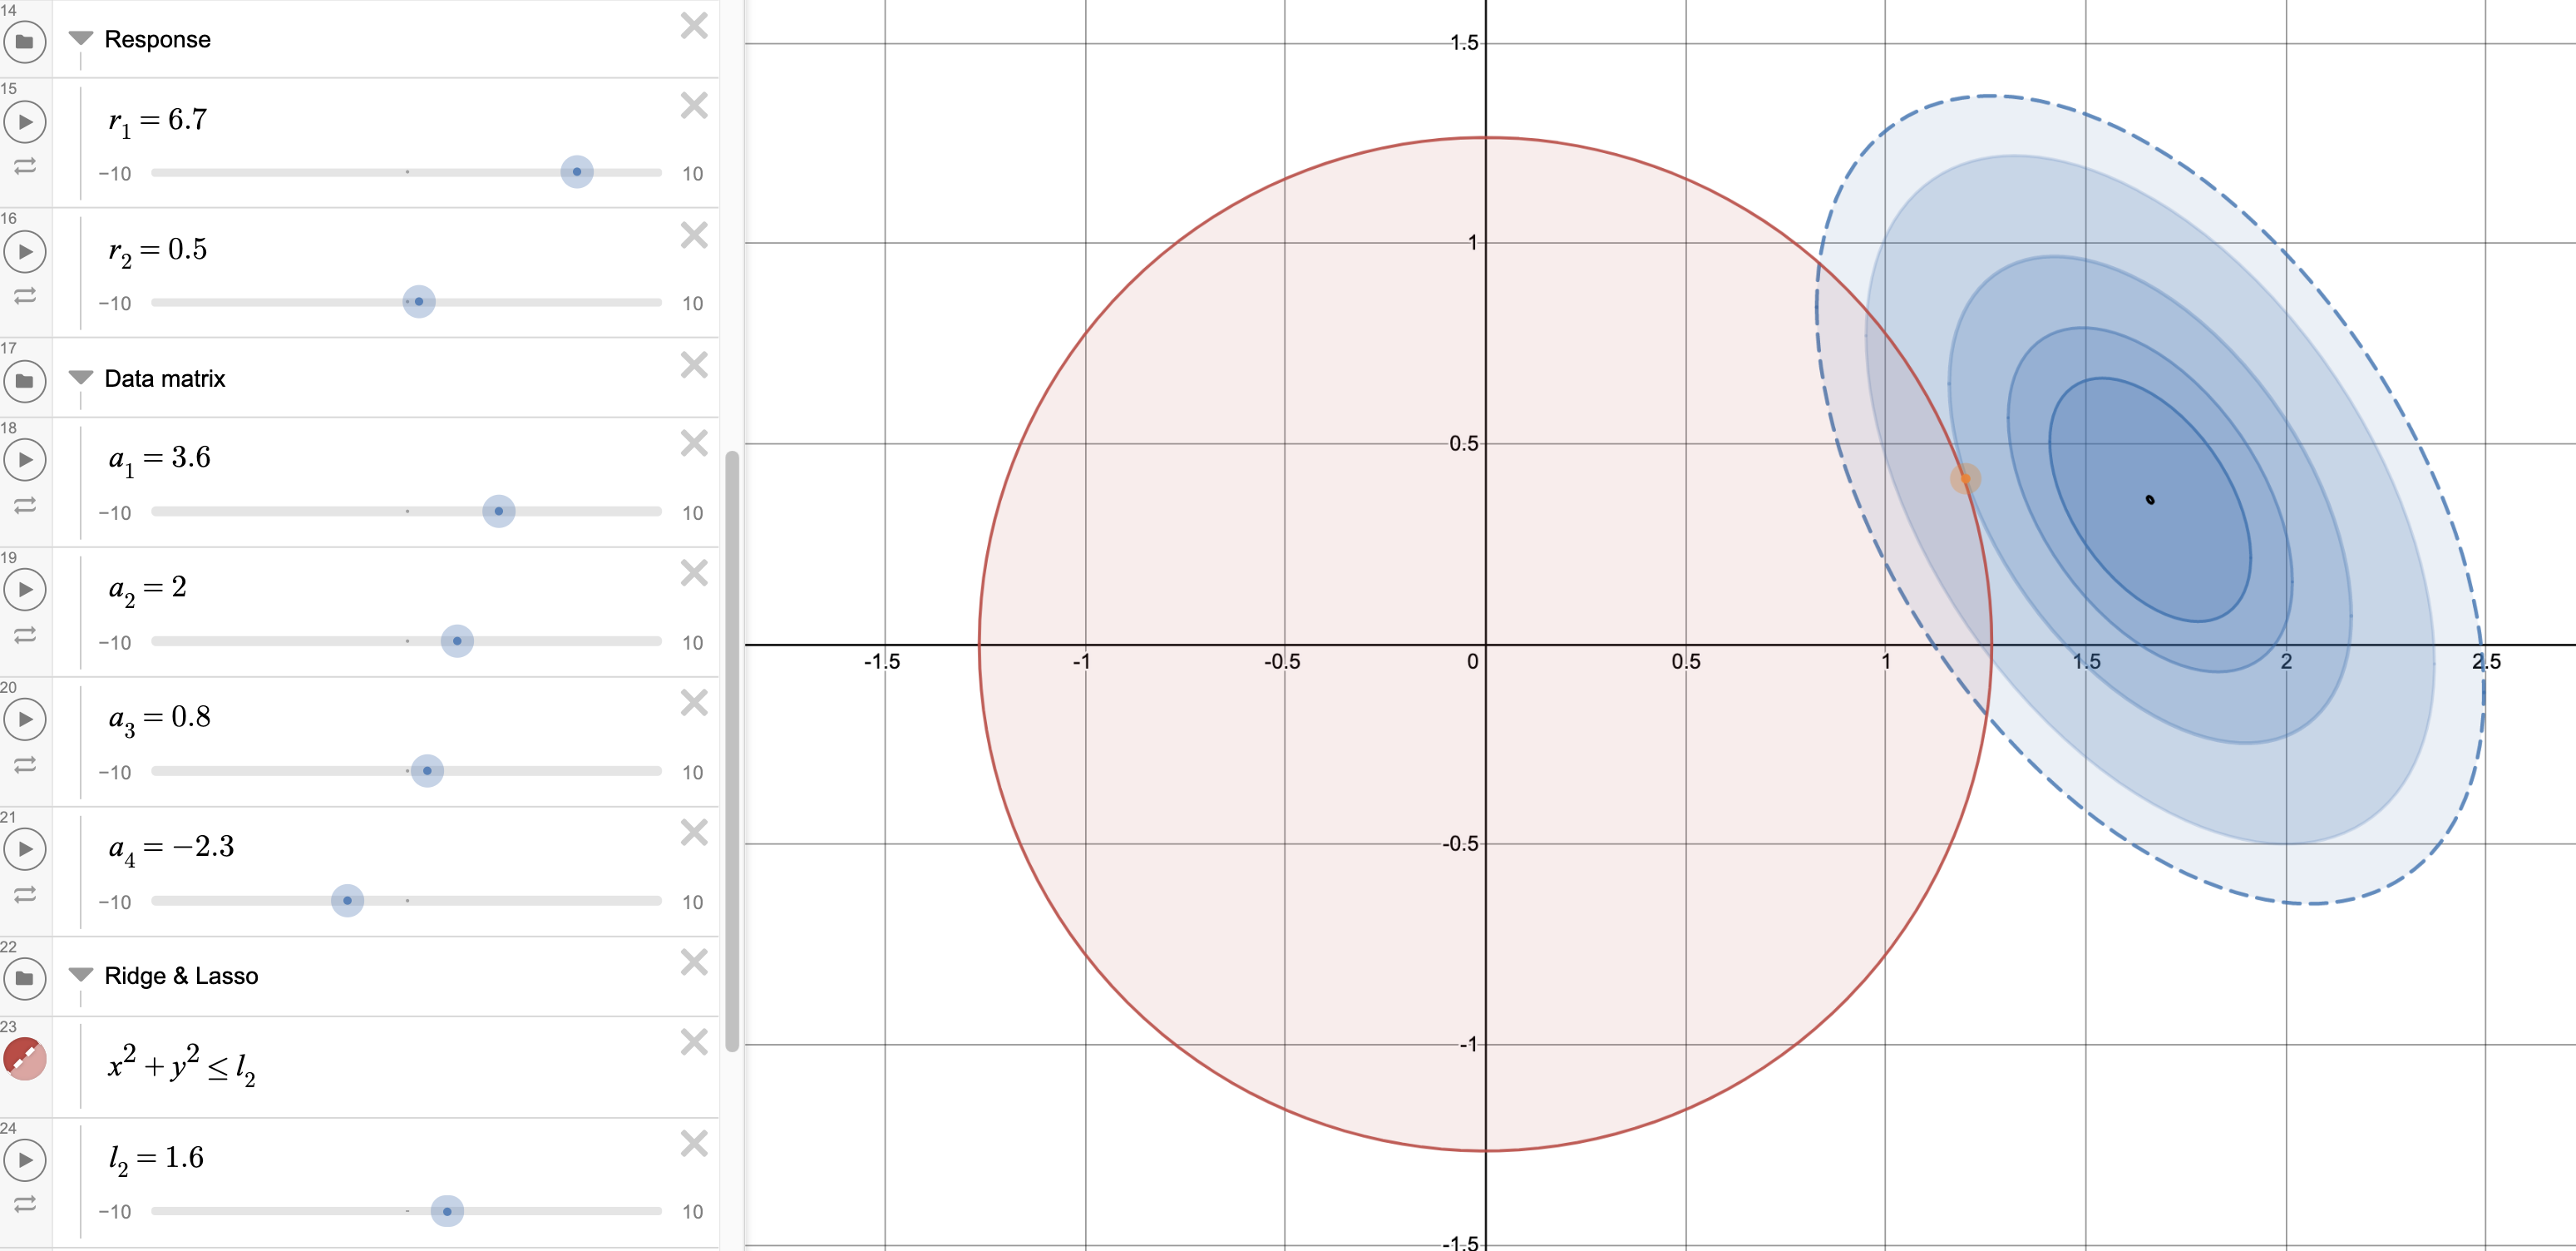
\includegraphics[width=1\textwidth]{ridge3.png}
\caption{Синим цветом показаны линии уровня целевой функции $ z((\beta_1,\beta_2)^\mathrm{T}) = \|\bm y - \X \betaa\|^2$, черная точка --- её безусловный минимум, который достигается на МНК решении. Однако это не будет решением по методу гребневой регрессии: теперь искать решение мы можем только внутри красного круга, радиус которого определяется параметром $\lambda$. Исходя из рисунка, минимум целевой функции при заданном ограничении достигается в оранжевой точке.}
\label{fig:rid_des}
\end{figure}

\subsection{Lasso}
По аналогии с задачей гребневой регрессии, которая может быть сформулирована как задача (\ref{eq:rid2}), можно рассмотреть такую задачу:
\begin{equation}
\label{eq:las}
\betah_{\text{lasso}}(\lambda) = \argmin_{\betaa}{\|\bm y - \X\betaa\|^2_2 \text{, т.ч. } \|\betaa\|_1 \leqslant \lambda}, \quad \lambda >0.
\end{equation}
Как можно видеть, изменилась только норма у ограничения $\|\betaa\|$; теперь рассматривается ограничение не на сумму квадратов, а на сумму модулей. Это влияет на вид множества ограничений: если раньше оно представляло из себя шар (см. рис \ref{fig:rid_des}), то теперь это ромб (в двумерном случае), размер которого также увеличивается с увеличением параметра $\lambda$.
\begin{figure}[]
\centering
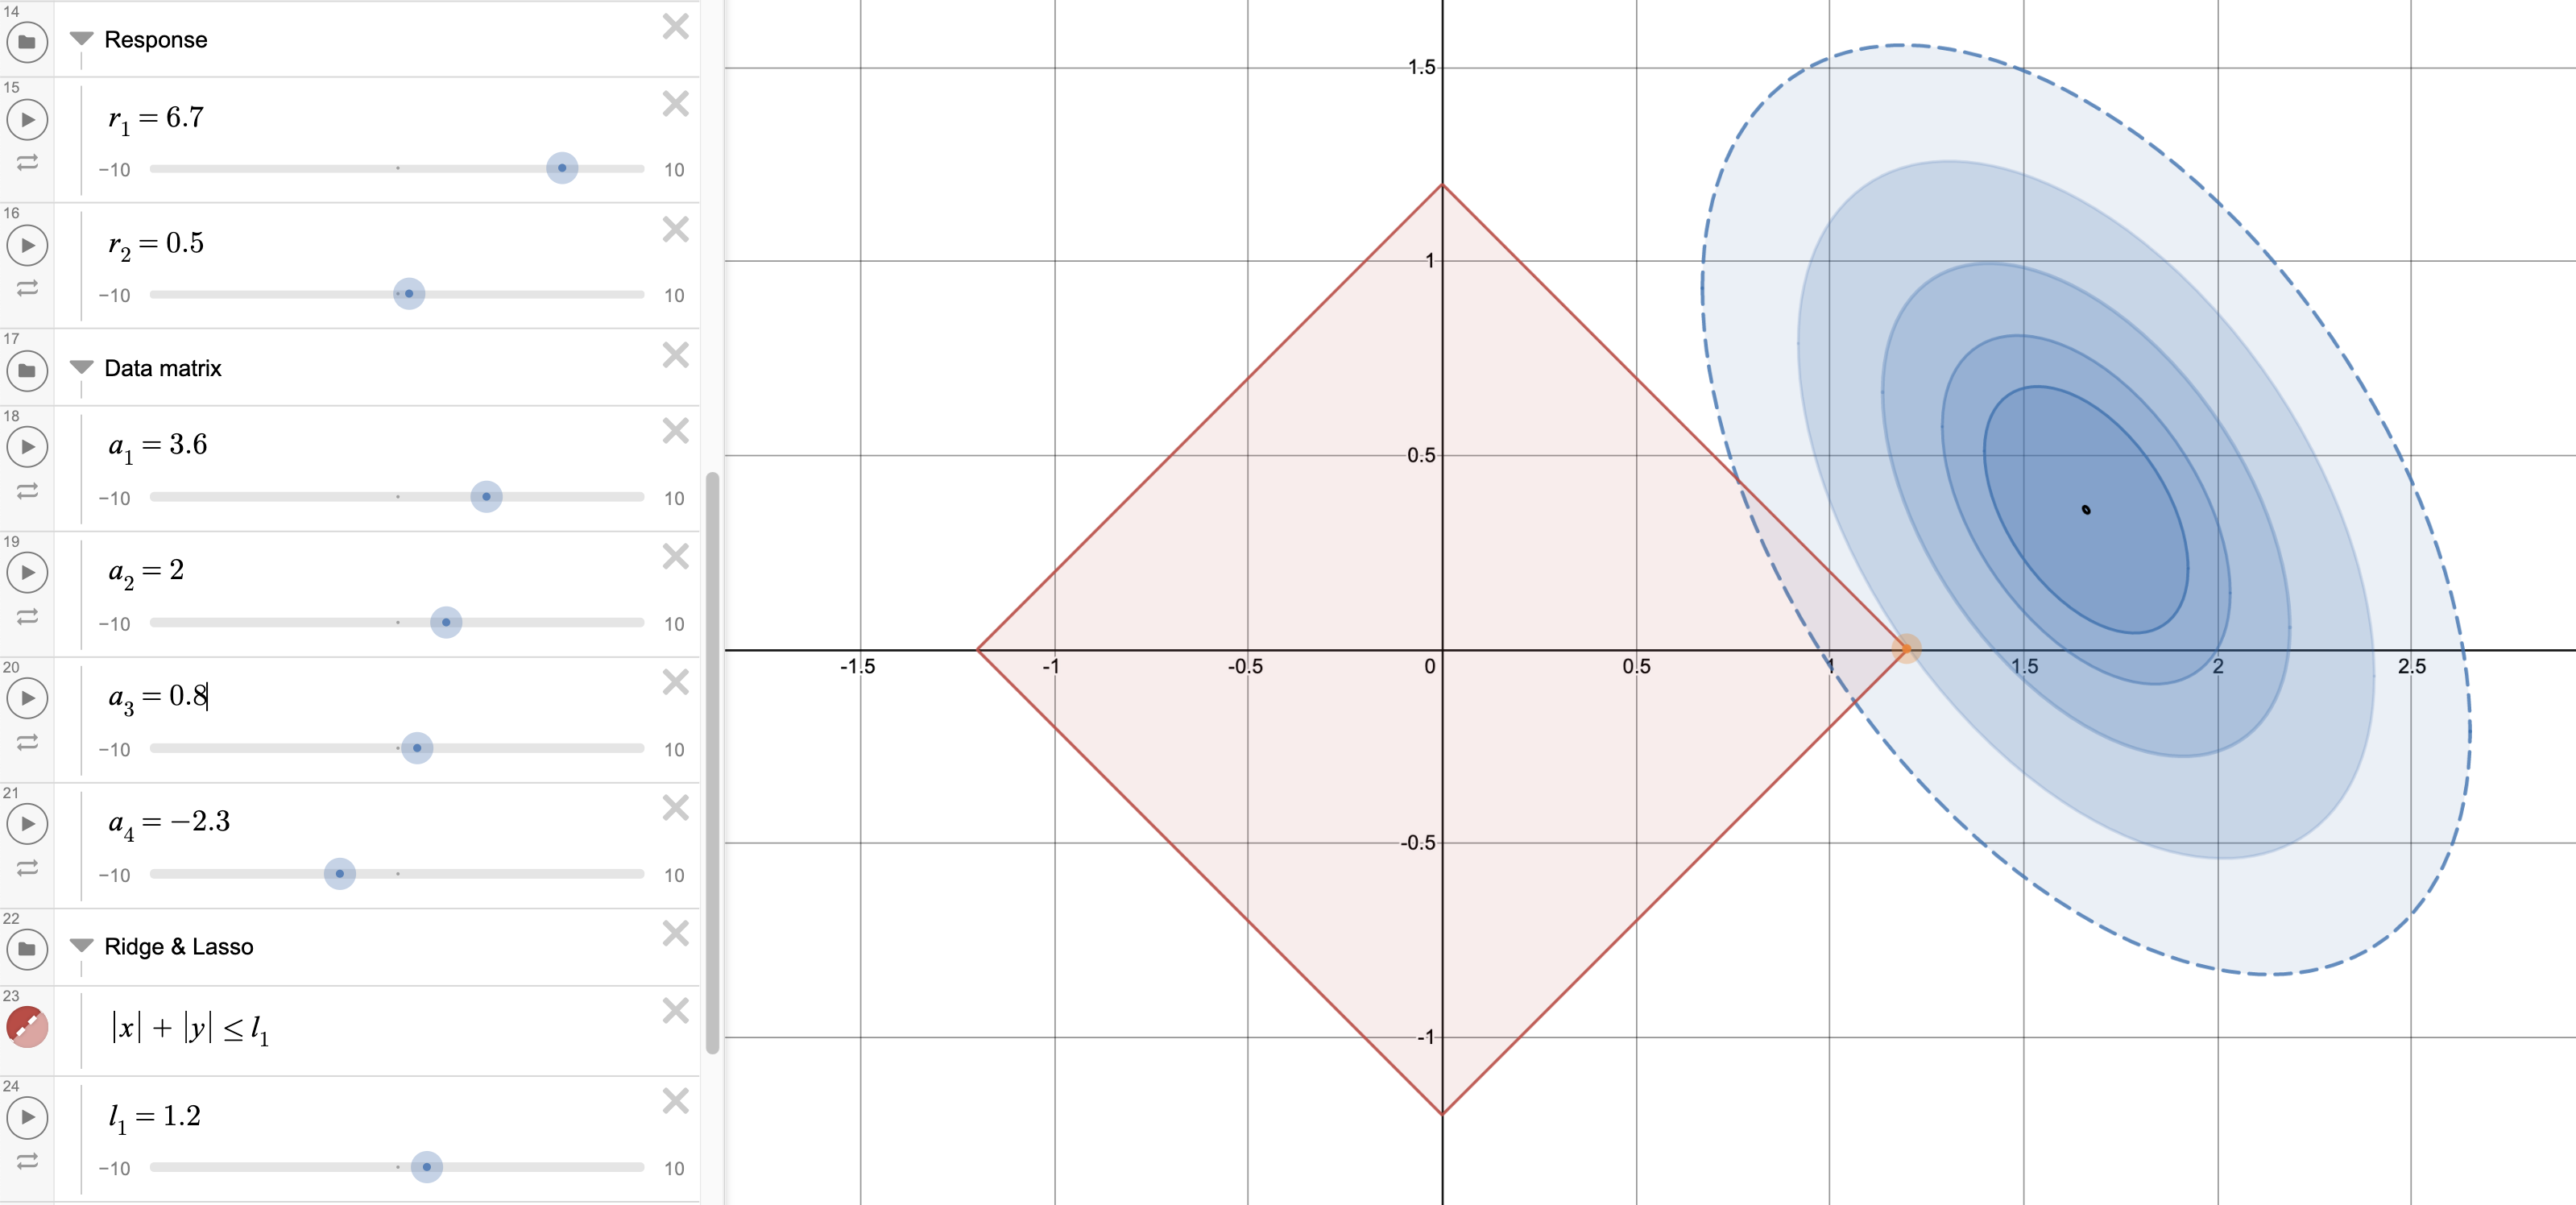
\includegraphics[width=1\textwidth]{lasso1.png}
\caption{Синим цветом показаны линии уровня целевой функции $ z((\beta_1,\beta_2)^\mathrm{T}) = \|\bm y - \X \betaa\|^2$, черная точка --- её безусловный минимум, который достигается на МНК решении. Решение по методу lasso показано оранжевой точкой: видно, что благодаря <<острому>> множеству ограничений, приходим к решению, у которого одна из координат --- нулевая. Решение по методу lasso отмечено оранжевой точкой.}
\label{fig:rid_des}
\end{figure}

Благодаря геометрическим особенностям нового множества ограничений $\|\betaa\|_1 \leqslant \lambda$ (см. двумерный пример на рис. \ref{fig:rid_des}), в результате решения задачи получаем вектор $\betah_{\text{lasso}}$, у которого некоторые компоненты равны нулю. С увеличением $\lambda$ некоторые координаты перестают быть нулевыми, а при $\lambda =+ \infty$ получаем классическое МНК-решение.

\paragraph{Особенности $\betah_{\text{lasso}}$}
Чаще всего отмечают два главных достоинства метода lasso:
\begin{enumerate}
	\item Уменьшение MSE;
	\item Увеличение интерпретируемости модели.
\end{enumerate}

Первое обусловлено тем, что опять же рассматриваем смещённую оценку, а наилучшее значение MSE достигается на компромиссном значении $\lambda$. 

Второе: имеется ввиду простота итоговой модели. Объясняется обнулением некоторых координат $\betah_{\text{lasso}}$: получается, что количество признаков, влияющих на ответ в полученной модели контролируется с помощью параметра $\lambda$. При небольших значениях $\lambda$ и, соответственно, малом количестве значимых признаков (тех, коэффициент при которых не равен нулю), модель становится легко интерпретируемой. При малых $\lambda$ будем иметь большее смещение, так что обычно параметр всё равно выбирается с помощью кросс-валидации, а не выбором <<удобного>> для интерпретации значения $\lambda$.

У данного метода так же есть и лимитации. Несмотря на то, что благодаря введённому ограничению (и, как следствие, уменьшению числа значимых признаков) появляется возможность рассмотрения случая $p>n$, адекватной оценки может не получится. 
Большинство теоретических результатов относительно сходимости решений lasso к истинному значению $\betaa$ основаны на том, что \textbf{сам вектор $\betaa$ является разреженным}, то есть имеет только небольшую долю ненулевых координат (например, задача с $n = 100, p = 40000$, а число значимых признаков составляет порядка $10$ признаков; ясно, что ни одна из данных ранее задач не привела бы к адекватному решению, но есть шанс, что lasso с этой задачей справится). 

\paragraph{Особенности нахождения оценки}
В отличие от МНК- и Ridge-оценок, явного решения у задачи lasso нет. В то же время, благодаря возможности переформулировки данной задачи в задачу квадратичного программирования,\footnote{и многим другим улучшениям, о которых здесь не будем распространяться, смотрите документацию и статьи к библиотеке \texttt{glmnet} на R или Python} у неё есть очень быстрая реализация в пакете \texttt{glmnet} --- решение для отдельного $\lambda$ вычисляется со скоростью, сопоставимой со скоростью вычисления МНК-оценки; также очень быстро вычисляется множество решений на сетке значений $\lambda$ (если полученное решение соответствует началу или концу построенной сетки, следует сдвинуть границы --- может оптимальное решение окажется там).

\section{Отбор признаков}
\label{sec:sel}

Как отмечалось в предыдущем разделе, в результате применения метода lasso получается вектор коэффициентов с большим количеством нулей, что приводит к итоговой модели с малым числом признаков. По сути, осуществляется процедура \textit{отбора признаков}. В этом разделе мы обсудим критерии выбора модели, а также ещё несколько подходов к решению задачи отбора признаков для модели.

\subsection{Критерии выбора модели}
\label{sec:crit}
Часто происходит так, что в рассмотрение берётся некоторый конечный набор моделей, а от статистика требуется выбрать наилучшую в некотором смысле модель.\footnote{например, модель линейной регрессии со всеми признаками или же модель, где признаков меньше и они выбраны на основании мнения экспертов} Выбор критериев зависит от предположений и конечной цели.

Итак, предположим, что есть некоторое семейство построенных моделей $\{\mathcal M_i\}_{i \in I}$. Хотим выбрать лучшую модель $\mathcal M^*$ для предсказания. Перечислим далее некоторые подходы к решению этой задачи.

\begin{itemize}
	\item Кросс-валидация:
	\begin{itemize}
		\item \textbf{leave-one-out CV }
		
		\textit{Строим модель для всех элементов выборки, кроме одного. Считаем на нём ошибку предсказания. Проделываем то же самое для каждого элемента выборки. Берём среднее по всем ошибкам.}
		\item \textbf{$k$-fold CV}
	
	\textit{Пример для $k = 5$: случайным образом разбиваем выборку на 5 частей. Строим модель по четырём частям и считаем ошибку на пятой нетронутой. Делаем так для 5 возможных комбинаций (1,2,3,4 и 5; 1,2,3,5 и 4; $\ldots$) и считаем среднюю ошибку по всем <<фолдам>>.}
	\end{itemize}
	\item Информационные критерии и $R^2$
		\begin{itemize}
	\item \textbf{AIC и BIC}
	
	Два стандартных критерия, которые используются не только в регрессионных моделях.
	
	Пусть $\mathcal L(\X; \mathcal M_i)$ --- максимум (по параметрам распределения) функции правдоподобия для модели $\mathcal M_i$, $p_i$ - число параметров в модели $i$. Тогда

	$$
	\mathrm{AIC}_i = 2p_i - 2\ln{\mathcal L(\X; \mathcal M_i)};
	$$
	$$
	\mathrm{BIC}_i = p_i\ln{n} - 2\ln{\mathcal L(\X; \mathcal M_i)}.
	$$
 Они представляют из себя функцию правдоподобия выборки с поправкой-штрафом, зависящей от числа параметров и размера выборки. Исходя из вида критериев, чем меньше значение, тем лучше; выбирается модель, у которой BIC или AIC наименьший.\footnote{нельзя забывать, что полученные значения зависят от выборки, то есть представляют из себя случайные величины; если значения AIC и BIC близки, то однозначного вывода отсюда сделать не получится}
 
 В BIC штраф за число параметров в модели больше. Так как в формуле участвует функция правдоподобия $\mathcal L(\X; \bm \theta)$, мы должны принять некоторое предположение о распределении выборки.
	\item \textbf{$R^2$}
	
	\textit{С увеличением числа признаков коэффициент детерминации $R^2$ только увеличивается, поэтому может привести к переобученной модели.
}	\item \textbf{$\text{adj.}R^2$}
	
	\textit{Здесь уже накладывается некоторый штраф за размерность пространства параметров.}
	\end{itemize}
\end{itemize}

\subsection{Отбор признаков в регрессии}

В разделе про методы регуляризации \ref{sec:reg} уже осветили один из способов снижения размерности пространства признаков --- lasso. В этом разделе кратко расскажем о классических методах: best subset selection, а также forward- и backward- subset selection.

\paragraph{Best subset selection}
Если имеется $p$ признаков, наивный вариант --- рассмотреть все возможные модели с $\tilde p = 1$ признаком, $\tilde p = 2$, и так далее до $\tilde p = p$, а затем выбрать наилучшую с помощью критериев из предыдущего раздела, \ref{sec:crit}. Количество таких моделей будет равно $2^p$. Если для примера взять $p = 20$, получим, что $2^p = 1,048,576$. Это уже довольно большое число моделей. При $p > 40$ данный подход становится затруднительным даже для построения МНК-оценок.

Также заметим, что из-за рассмотрения большого числа моделей, применение метода best subset selection может привести к проблеме переобучения (происходит подгонка модели под тренировочную выборку).

\paragraph{Forward и backward subset selection}
Также существуют и <<жадные>> альтернативы методу best subset selection. Один из вариантов (\textit{Forward subset selection}) состоит в выборе наилучшей модели с одним признаком, а затем последовательное добавление признаков, которые оказывают наилучшее влияние на критерий выбора. В итоге получаем $p(p+1)/2$ моделей.\footnote{для $p = 20$ получаем $210$ моделей --- значительно меньше, чем у best subset} Далее можем выбирать на основании желаемого числа признаков или опять же на основании тех же критериев. 

Аналогично можно начинать со всех признаков и последовательно удалять по одному, пока не придём к модели с одним признаком (\textit{Backward subset selection}). Замечание: в случае, когда $p>n$ и считаются МНК-оценки (к примеру), метод Backward subset selection уже не сработает, так как нет возможности начать процедуру с полного пространства признаков.




\section{Источники и рекомендуемая литература}

\begin{itemize}
	\item ESL (Elements of Statistical Learning) --- Hastie, Tibshirani, Friedman;
	\item ISLR (An Introduction to Statistical Learning) --- James, Witten, Hastie, Tibshirani;
	\item Лекции Н.Э. и А.И., СтатМод;
	\item Лекции Воронцова по ML;
	\item Лекции Larry Wasserman --- Statistical Learning;
	\item All of Statistics --- Larry Wasserman.
		\end{itemize}



\end{document}


